\documentclass[a4paper]{article}
\usepackage[x11names,svgnames]{xcolor}
\usepackage[T1]{fontenc}
\usepackage[utf8]{inputenc}
\usepackage[francais]{babel}
\usepackage{amsmath}
\usepackage{graphicx}
\usepackage{subfigure}
\usepackage[colorinlistoftodos]{todonotes}
\usepackage{array}
\usepackage{setspace}
\usepackage{fullpage}
\usepackage[justification=centering]{caption} % necessaire pour caption longue de plus d'une ligne.
\usepackage{hyperref} 
%\pdfcompresslevel=9 
\hypersetup{ 
     colorlinks=true, %colorise les liens 
     breaklinks=true, %permet le retour àˆ la ligne dans les liens trop longs 
     urlcolor= blue,  %couleur des hyperliens 
     linkcolor= Blue4, %couleur des liens internes crééŽs, 
}
\usepackage{listings}
\lstset{
language=python,
commentstyle=\textit,
basicstyle=\ttfamily\color{Black},
keywordstyle=\color{DarkRed},
commentstyle=\color{Blue3}\normalfont,
}
\newcommand{\cin}[1]{\lstinline{#1}}

% Francisation
\addto\captionsfrench{\renewcommand{\tablename}{{\scshape Tab.}}}

% Colonnes de largeur fixe
\newcolumntype{L}[1]{>{\raggedright\let\newline\\\arraybackslash\hspace{0pt}}m{#1}}
\newcolumntype{C}[1]{>{\centering\let\newline\\\arraybackslash\hspace{0pt}}m{#1}}
\newcolumntype{R}[1]{>{\raggedleft\let\newline\\\arraybackslash\hspace{0pt}}m{#1}}


\def\thesection{Question \arabic{section}}
\def\thesubsection{\alph{subsection}}

\onehalfspacing

% Bibliographie
\bibliographystyle{ieeetr}


\title{TP3 - IMN530}

\author{FOUQUET, Jérémie et MÉTHOT, Vincent}

\date{28 avril 2014}

\begin{document}
\maketitle

\section{IRM fonctionnelle}

Plusieurs outils d'analyse existent pour traiter des données d'IRMf. Nous avons choisis de les utiliser directement plutôt que de les implémenter en python. Deux suites logicielles ont retenu notre intérêt (puisque nous les connaissons déjà), soit FSL [http://fsl.fmrib.ox.ac.uk/fsl/fslwiki/] et AFNI [http://afni.nimh.nih.gov/], qu'il faudra avoir installé pour faire fonctionner le script associé à ce numéro (Q1_IRMf.sh).

\subsection{Étapes de reconstruction}

Il faut garder à l'esprit qu'à chaque étape de reconstruction, il est fortement conseillé d'inspecter visuellement les données. Dès leur réception, on a visuellement inspecté plusieurs tranches de \emph{fmri.nii} à plusieurs temps pour s'assurer que les artéfacts n'étaient pas trop important et que la correction de mouvement n'était pas nécessaire (voir Fig. \ref{fmri_anatomist}, comme mentionné dans la question. De plus, nous avons effectué une transformée de Fourier des séries temporelles.

\begin{figure}[h]
   \caption{\label{fmri_anatomist} Inspection visuelle de fmri.nii dans anatomist. On peut inspecter plusieurs tranches pour tous les points temporels à l'aide des deux curseurs à droite, comme dans un film.}
   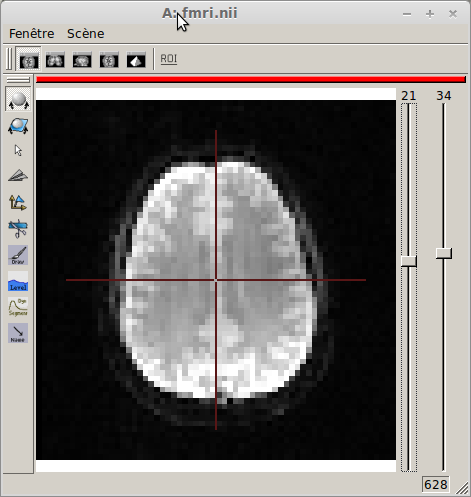
\includegraphics[width=0.7\textwidth]{fmri_anatomist}
\end{figure

% Faire plein de figures pour montrer les observations...



\subsection{Segmentation}

\subsection{Zones d'activation}

\section{IRM de diffusion}

\subsection{Estimation des tenseurs}

\subsection{FA et ADC}

\subsection{Tractographie}

\section{Fusion}

\subsection{Justification}

\subsection{Connectivité des zones fonctionnelles}

\section{Bonus}

\subsection{FA et ADC}

\subsection{Tractographie avec Dipy}


\end{document}